\documentclass[11pt,a4paper,oneside]{book}

\usepackage[english]{babel}

%%\usepackage{times}
\usepackage{helvet}
\renewcommand*\familydefault{\sfdefault} %% Only if the base font of the

\usepackage[T1]{fontenc}
\usepackage[latin1]{inputenc}
\usepackage{amsmath}
\usepackage{amssymb}
\usepackage{graphicx}
\usepackage{longtable}
\usepackage{multirow}
\usepackage{tabularx}
\usepackage{fancyhdr}
\usepackage{float}
\usepackage[Sonny]{fncychap}
\usepackage{hyperref} % Indice nel pdf, da togliere per la stampa perché crea conflitto.
\usepackage{subfigure}
\usepackage{pdfpages}
\usepackage{titlesec}
\usepackage{rotating}
\usepackage{color}
\usepackage{gensymb}
%\usepackage[citestyle=numeric,hyperref,natbib=true,backend=bibtex]{biblatex}
%\renewcommand\nameyeardelim{, }


%\addbibresource{Bibliografia}
%\pagestyle{empty}

\usepackage{geometry}
 \geometry{
 a4paper,
 total={210mm,297mm},
 left=30mm,
 right=35mm,
 top=30mm,
 bottom=40mm,
 }


\newcommand{\tb}{\textsubscript}
\newcommand{\ts}{\textsuperscript}
\newcommand{\bs}{\textbackslash}


\graphicspath{{./immagini/}}


\begin{document}



%\begin{titlepage}
\thispagestyle{empty}


\begin{center}
\text{\large Institute for Renewable Energy}
\end{center}

\begin{figure}[h]
     \begin{center}
         
\includegraphics[width=0.5\textwidth]{logo}
     \end{center}
     \label{fig:logo_uni}
 \end{figure}

\vspace{4 cm}

\begin{center} 
%\text{\LARGE Usefulness of Landsat data for monitoring vegetation changes}\\
\text{\Huge  TypeDLT}\\
\vspace{0.5 cm}
\text{\Huge Tutorial}\\

\end{center}

%\vspace{1.2 cm} 
% %\rule{1.0\textwidth}{0.5pt}
%\hrule \
%\vspace{0.5 cm}
% \begin{center}
%\textsc{3D Finite Volume Method applied to Heat-Transfer}\\
%\end{center}
%\hrulefill \

\vspace{5 cm}

\begin{tabular}{lr}  
 
Contacts	&			\\

Giuseppe De Michele		& \href{mailto:giuseppe.demichele@eurac.edu}{giuseppe.demichele@eurac.edu}	 			\\
Ulrich Filippi Oberegger		&	\href{mailto:ulrich.filippi@eurac.edu}{ulrich.filippi@eurac.edu}				\\
Luca Baglivo 		&		\href{mailto:luca.baglivo@eurac.edu}{luca.baglivo@eurac.edu}			\\
\end{tabular}

\end{titlepage}


%DA DECOMMENTARE AL MOMENTO DELLA STAMPA INTEGRALE
%\newpage
%\null
%\thispagestyle{empty}
%\newpage



%\fancyhead[LE,RO]{\scriptsize \rightmark} % 
%\fancyhead[LO,RE]{\scriptsize \leftmark}
%\fancyfoot[C]{\thepage}
%\renewcommand{\chaptermark}[1]{ %
%\markboth{\thechapter.\ #1}{}}

\pagestyle{fancy} 
\fancyhf{}%cancella tutti i campi 
%\headsep 2cm %altrimenti si sovrappone il testo alla hdr 
\fancyhead[R]{\includegraphics*[width=3cm]{logo}% non c'è l'ambiente figure.
} 
\fancyhead[L]{\large \textsc{TypeDLT - User Guide} }
\fancyfoot[C]{\thepage}
\renewcommand{\headrulewidth}{0.1pt}

%\pagestyle{fancy}
%\fancyhead[RO]{{ \footnotesize \rightmark}}
%\fancyfoot[RO]{\thepage}
%\fancyhead[LE]{{ \footnotesize \leftmark}}
%\fancyfoot[LE]{\thepage}
%\fancyhead[LO,RE]{}
 
%%\renewcommand{\footrulewidth}{0.1pt}

%\frontmatter

%\tableofcontents
%\listoffigures
%\listoftables

%\input{chapter/sommario}


%\mainmatter

\begin{titlepage}
\thispagestyle{empty}


\begin{center}
\text{\large Institute for Renewable Energy}
\end{center}

\begin{figure}[h]
     \begin{center}
         
\includegraphics[width=0.5\textwidth]{logo}
     \end{center}
     \label{fig:logo_uni}
 \end{figure}

\vspace{4 cm}

\begin{center} 
%\text{\LARGE Usefulness of Landsat data for monitoring vegetation changes}\\
\text{\Huge  TypeDLT}\\
\vspace{0.5 cm}
\text{\Huge Tutorial}\\

\end{center}

%\vspace{1.2 cm} 
% %\rule{1.0\textwidth}{0.5pt}
%\hrule \
%\vspace{0.5 cm}
% \begin{center}
%\textsc{3D Finite Volume Method applied to Heat-Transfer}\\
%\end{center}
%\hrulefill \

\vspace{5 cm}

\begin{tabular}{lr}  
 
Contacts	&			\\

Giuseppe De Michele		& \href{mailto:giuseppe.demichele@eurac.edu}{giuseppe.demichele@eurac.edu}	 			\\
Ulrich Filippi Oberegger		&	\href{mailto:ulrich.filippi@eurac.edu}{ulrich.filippi@eurac.edu}				\\
Luca Baglivo 		&		\href{mailto:luca.baglivo@eurac.edu}{luca.baglivo@eurac.edu}			\\
\end{tabular}

\end{titlepage}

\tableofcontents
\chapter*{Introduction}
TypeDLT is a new component for TRNSYS able to perform daylighting simulation of complex fenestration system using RADIANCE. The new type has been developed by the Institute of Renewable Energy of EURAC within the EU FP7 Project CommONEnergy. \\
The TypeDLT expand the capabilities of TRNSYS allowing to take in account also the visual comfort in order to have a overall vision of the behaviour of the building in terms of energy balance but also thermal and visual comfort. It is also possible the connection of TypeDLT with other types on the TRNSYS deck in order to define custom shading controls. 
\\
\\
The following document explain how to start with the daylighting simulation within TRNSYS. 
\chapter{TypeDLT}
\section{Description and functionality}
The new TypeDLT (DayLightTing), written in the C\texttt{++} programming language, performs the Three-Phase Method for dynamic, climate-based daylighting simulations of CFS taking in input the BSDF data \cite{bsa}.
The TypeDLT receives the following inputs from the weather file:
\begin{itemize}
\renewcommand{\labelitemi}{\tiny$\blacksquare$}
\item Latitude and longitude
\item Month, day of the month, hour of the day
\item Direct normal illuminance
\item Diffuse horizontal illuminance
\end{itemize}
In this way it can identify the building location (and thus calculate the sun path) and the information for the climate-based analysis. The following parameters are set in the Type's control panel:
\begin{itemize}
\renewcommand{\labelitemi}{\tiny$\blacksquare$}
\item Zone ID, thermal zone for which the shading system is controlled
\item Control, determining which BSDF is used
\end{itemize}
These parameters are necessary to identify the thermal zone where CFS are controlled, which CFS assigned to that zone are controlled, and which are the initial conditions for the simulation. A BSDF data file has to be provided for each shading state. In order to independently control a series of thermal zones, the TypeDLT can be added as functional block to the simulation model multiple times, with different parameters, inputs, and outputs.
The outputs of the Type are:
\begin{itemize}
\renewcommand{\labelitemi}{\tiny$\blacksquare$}
\item Maximum (or average, minimum) illuminance value over the sensors grid
\item Control, current shading state
\end{itemize}
The control algorithm, defined through a series of equations which can involve inputs and outputs of other Types, the Type56 and the TypeDLT are interlinked. Loops between Types can be formed. By default, TRNSYS performs iterations after each time step until all parameters, inputs and outputs of every Type have converged. Therefore, the main difference with other integrated software is the time-step interaction of the TypeDLT with the other Types contained into the TRNSYS deck. \\
The control algorithm is not incorporated into the TypeDLT, but implemented through the "Equation" functional blocks that TRNSYS offers by default. This has the big advantage that the TypeDLT does not need to be recompiled every time the control strategy has changed and can thus be reused more easily by the user.
This approach gives the maximum flexibility in the setting of a shading control strategy, since it is possible to test custom control algorithm taking in account all the main aspects of a sustainable design: energy saving, thermal and visual comfort, but with the detriment of calculation time.

\begin{figure}[h]
\centering
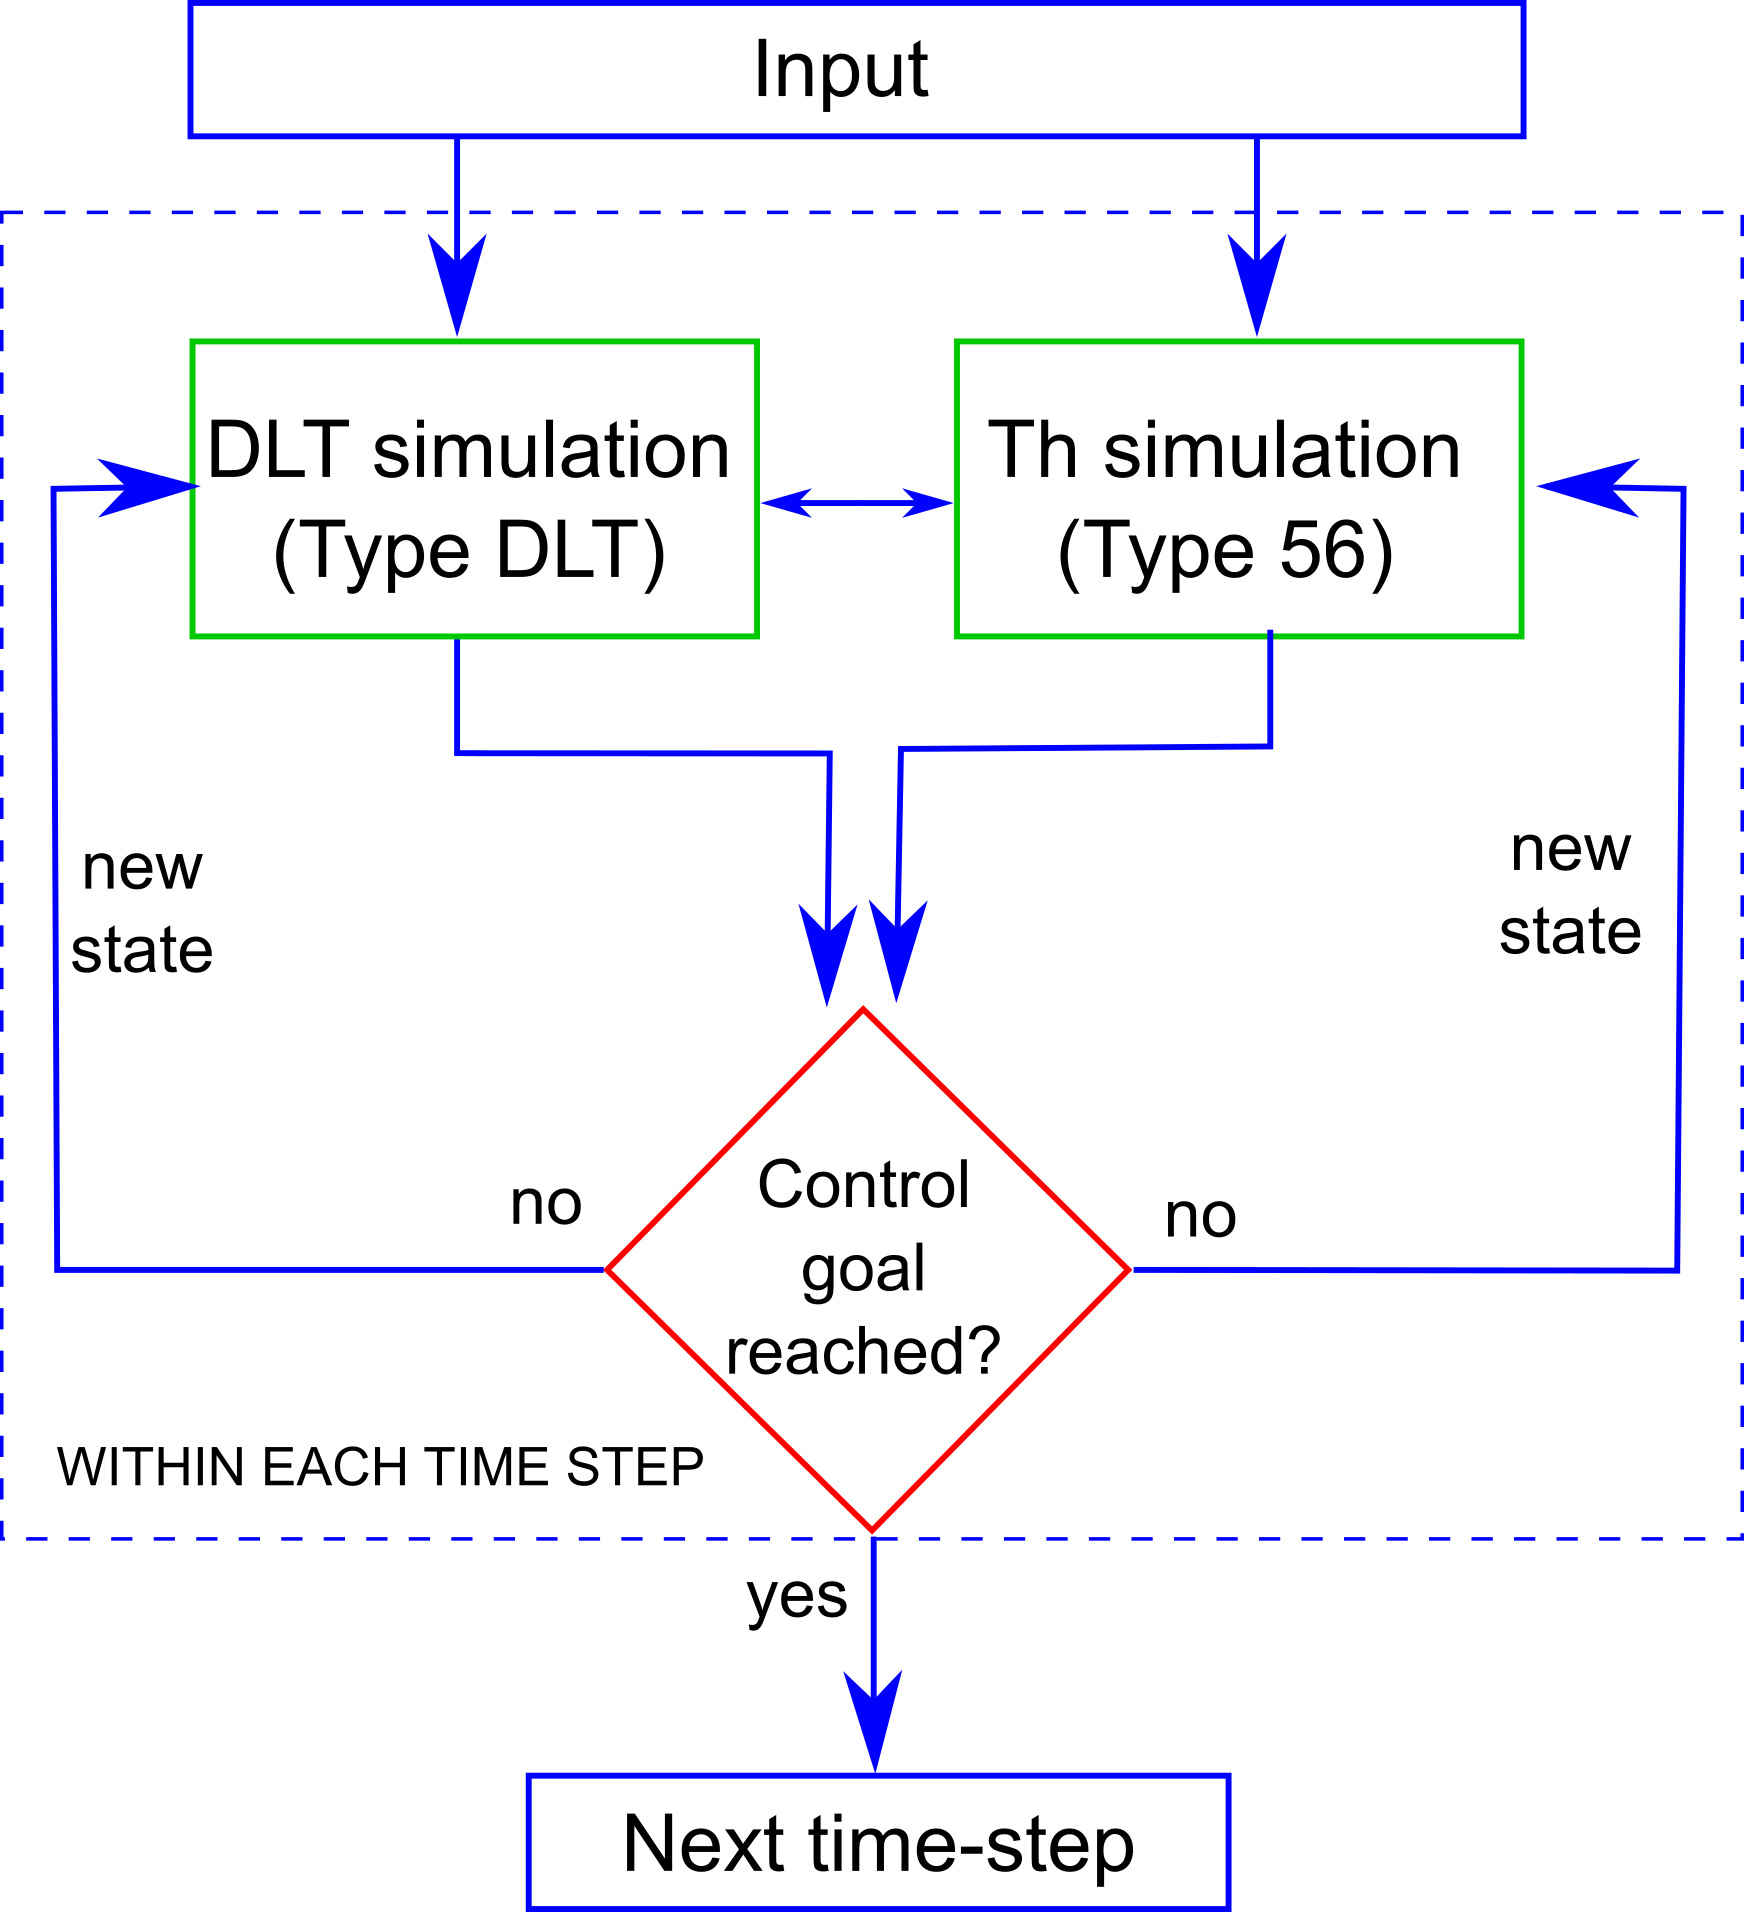
\includegraphics[width=0.7\textwidth]{control}
\caption{\label{img2:flow} Flow chart of the iteration process between daylighting and thermal simulation within each time step}
\end{figure}

Figure \ref{img2:flow} shows a typical workflow of the process. Both the daylighting (TypeDLT) and the thermal (Type56) simulations take their inputs. Then, the BSDF data and the Types' outputs are passed to a control "Equation" (a special functional block of TRNSYS in which an equation system can be defined) that modifies the shading states. By default, TRNSYS iterates until all Type outputs have reached convergence. Only then, it advances in time by performing the next time step.\\ 
At each time step the TypeDLT outputs can be shard with all the other types onto the TRNSYS deck (Figure \ref{img2:implem}), for example can be used for the artificial light calculations, in the control algorithm and/or passed to the Type56 as shading factor.

%\begin{figure}[h]
%\centering
%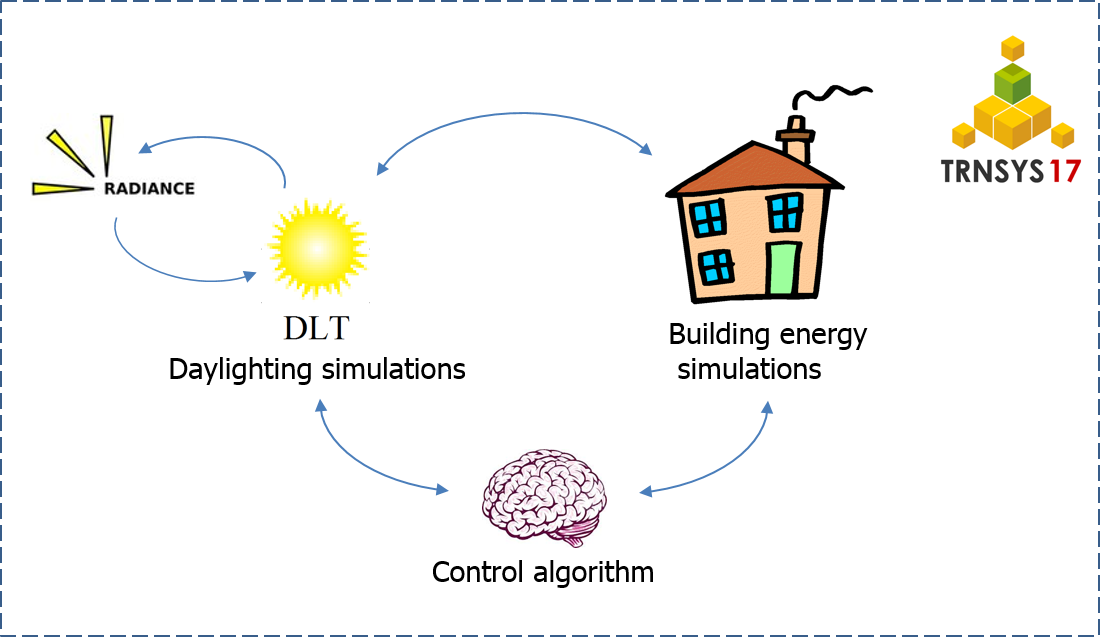
\includegraphics[width=0.9\textwidth]{deck}
%\caption{\label{img2:deck} Deck}
%\end{figure}

The advantages available by the use of TypeDLT are: 
\begin{itemize}
\renewcommand{\labelitemi}{\tiny$\blacksquare$}
\item Customized shading control based on: daylighting parameters, thermal parameters, weather file parameters or a combination of that
\item Use of the BSDF file as input data
\item Multi-zone daylighting analysis by adding more TypeDLT 
\item Easy calculation of artificial lighting usage
\item No limit in the complexity of the model geometry 
\item Complete overview of the CFS effects on building in terms of energy demand and thermal and visual comfort
\item Possibility to control up to 10 windows/group of windows with different strategies.
\end{itemize}

\begin{figure}[h]
\centering
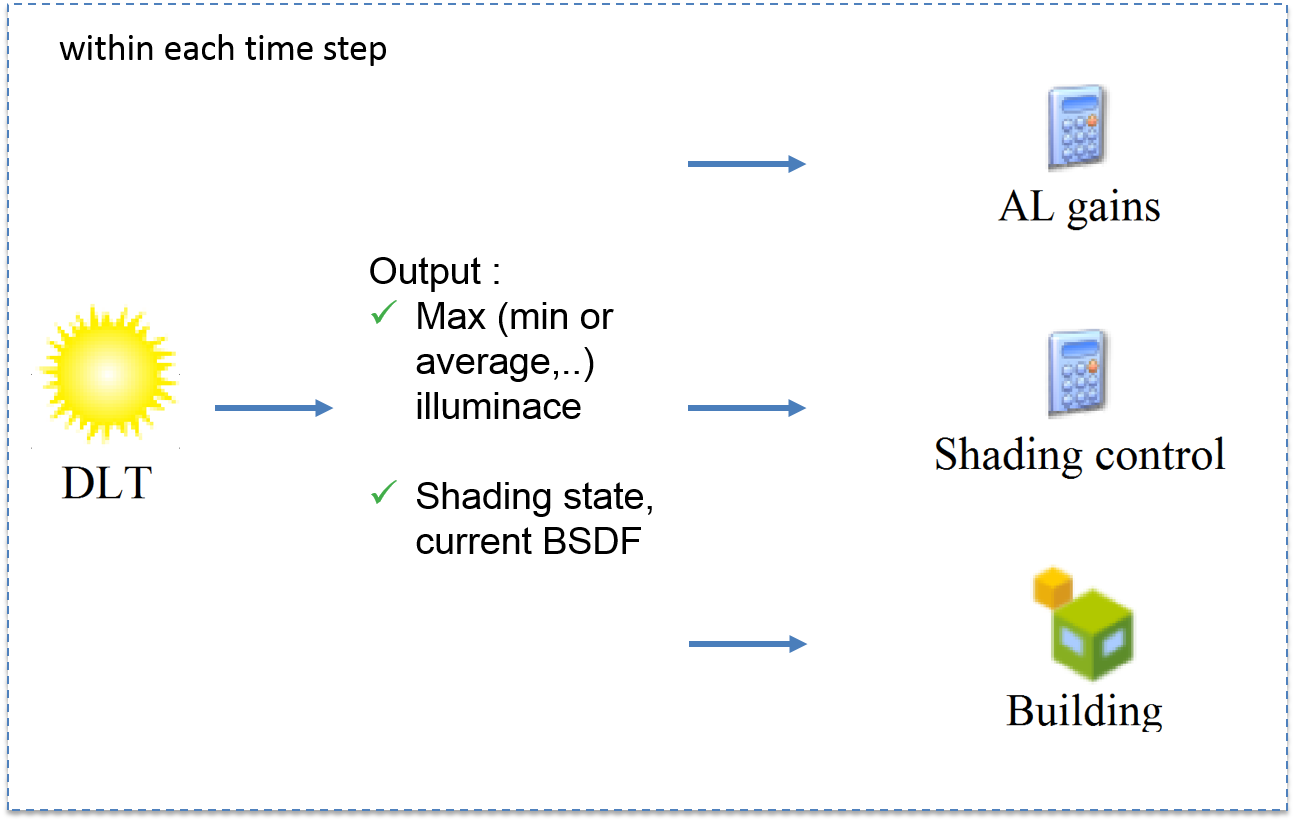
\includegraphics[width=0.7\textwidth]{implem}
\caption{\label{img2:implem} TypeDLT outputs and possible connection with other types}
\end{figure}

The disadvantages are due to:
\begin{itemize}
\renewcommand{\labelitemi}{\tiny$\blacksquare$}
\item Time consuming simulation
\item Not user-friendly simulation set-up
\end{itemize}

The hourly-based approach allows a complete information sharing between the TypeDLT and the rest of the Types over the TRNSYS deck at each time-step, on the other hand this strategy take a lot of time because a daylighting simulation is performed at each time-step slowing down the energy simulation with TRNSYS.\\
As explained in the following pages, the phase of set-up of the simulation take time if the user is not yet familiar with the procedure and required the use of different software.\\
The feature of a multiple shadings control within the same scene is currently under development, and will be available in next release.

\section{Installation}
Below is sorted the list of software required for the TypeDLT running. Keep in mind that those software are only suggested, except for Radiance, and the user is free to use an equivalent software that does the same job.

\subsection{Radiance}
Download the binary for Windows from \url{https://github.com/NREL/Radiance/releases} and run the exe. Install Radiance to (\textit{C:\textbackslash Radiance}).

\subsection{Perl environment for OS Windows}
A Perl interpreter is necessary to run Perl application on Windows. In fact, some of the functions used in Three-Phase Method are written in Perl programming language, therefore an interpreter is required. 
For this purpose is possible get the proper version of Perl from \url{http://strawberryperl.com/} install it and make sure to add the Perl executable directory to your PATH (the installers will optionally do this for you).

\subsection{TypeDLT}
Recompiling the DLT.dll file became necessary if you use a system different from Windows 8.1 64 bit, for which the TypeDLT has been compiled, or if the C\texttt{++} code has been modified.\\
For this step, the batch file \textit{compilation\_into\_dll.bat} is supplied. The batch file contains two lines of code that execute mingw32-g++.exe which creates the DLL starting from the C\texttt{++} code. Follow the steps below to use the batch file:
\begin{enumerate}
\item Install code::block from \url{http://www.codeblocks.org/downloads}.
\item Install mingw-get-setup.exe from \url{http://sourceforge.net/projects/mingw/files/latest/download?source=files} and install it in C: without space.
\item Open Environment variables (see \url{http://www.computerhope.com/issues/ch000549.htm} if you are not familiar with) add  
\begin{center}
\textit{C:\textbackslash MinGW\textbackslash bin}
\end{center} to the PATH as shown in figure \ref{img2:environment}.

\begin{figure}[h]
\centering
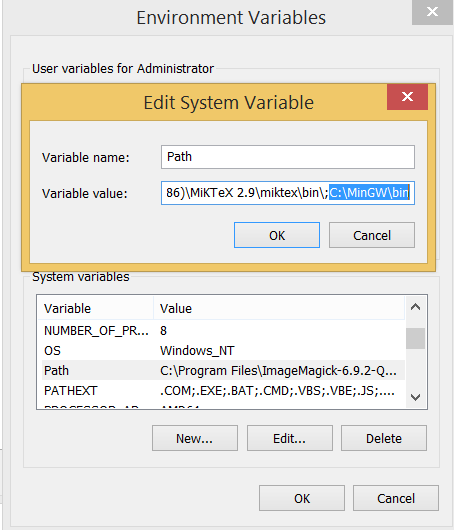
\includegraphics[width=0.5\textwidth]{environment}
\caption{\label{img2:environment} Environment variable setting}
\end{figure}


\item Open the Windows terminal following the steps:
\begin{itemize}
\item Type WinKey + R
\item Input "cmd"
\item Type Enter
\end{itemize}
\item Move into the MinGW folder with the command


 \begin{center}
  \textit{cd C:\textbackslash MinGW\textbackslash bin}   \end{center}  and run the command \begin{center}
  \textit{mingw-get install c++}  \end{center} 
as in Figure \ref{img2:mingw}.

\begin{figure}[h]
\centering
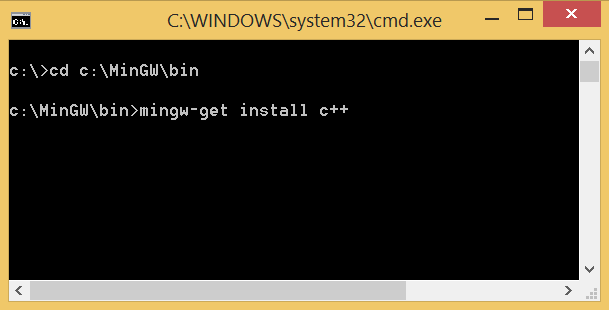
\includegraphics[width=0.6\textwidth]{mingw}
\caption{\label{img2:mingw} Terminal with the commands to launch}
\end{figure}

\item Launch the batch file \textit{compilation\_into\_dll.bat} within the folder that we provided you. This because the file needs other files contained in this folder.
\end{enumerate}



%In this batch file has to be changed the executable file path of mingw32-g++, setting the proper for your path at the beginning of batch file as shown in figure \ref{img2:dll}.

%\begin{figure}[h]
%\centering
%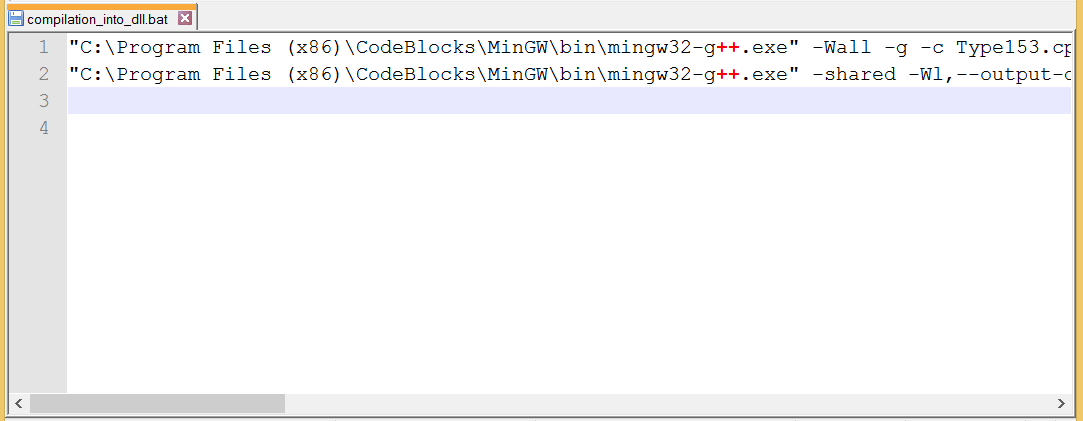
\includegraphics[width=0.7\textwidth]{dll}
%\caption{\label{img2:dll} Beginning of the compilation\_into\_dll.bat file.}
%\end{figure}

Once the DLT.dll is created the file has to be located in the TRNSYS folder \begin{center}
C:\textbackslash Trnsys17\textbackslash UserLib\textbackslash ReleaseDLLs \end{center}
The proforma files (.tfs and .btp) have to be placed in the proformas folder within an existing folder or in a new one, such as \begin{center}
\textit{ C:\textbackslash Trnsys17\textbackslash Studio\textbackslash Proformas\textbackslash mycomponent} 
\end{center}

\section{Tool Chain}
In order to carry on with the daylighting simulation it is necessary to prepare the daylighting model, manipulate some configuration files and retrieve the BSDF data.

\subsection{BSDF data generation - WINDOW 7.3}
The BSDF data can be generate through several methods: window modelling software (e.g. WINDOW 7.3), simulation programs (e.g. TrancePro or Radiance's "genBSDF") or measurements with a goniophotometer. In this section will be given an overview of the BSDF file creation with the software WINDOW 7.3.\\

The software WINDOW 7.3, developed by the LBNL in California, allows to define or calculate the BSDF data for standard system and parameters such as the Solar Heat Gain Coefficient (SHCG or g-value), heat transfer coefficient (U-factor) and visible transmittance (Tvis).\\
Within the Glazing System Library (Figure \ref{img2:window}) it is possible to create the fenestration system choosing the glass and the shade typology from the respective database, IGDB and CGDB. Figure \ref{img2:window} shows a system composed by a double pane glass with solar control and, as shading device, a system of louvre tilted at 30-degree tilt angle.
 
\begin{figure}[h]
\centering
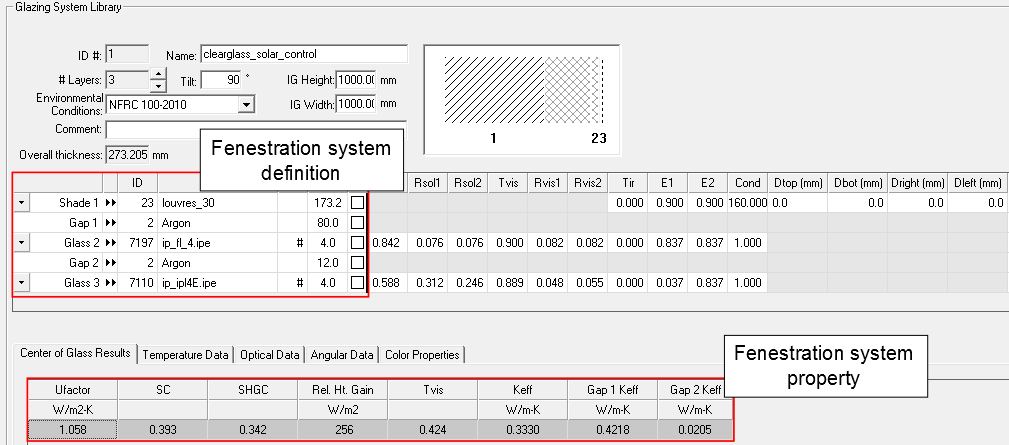
\includegraphics[width=0.8\textwidth]{windowsystem}
\caption{\label{img2:window} Glazing System Library }
\end{figure}

From the Shading Layer Library (Figure \ref{img2:shading}), it is also possible to assign a custom shading device choosing from the shading type: venetian blinds, homogeneous diffusing shade, woven shade, fritted shade. Then, for each typology, it is possible to choose geometric and optical parameters. WINDOW allows also to use BSDF data pre-calculated in the shading type by selecting "shade with XML data". 

\begin{figure}[h]
\centering
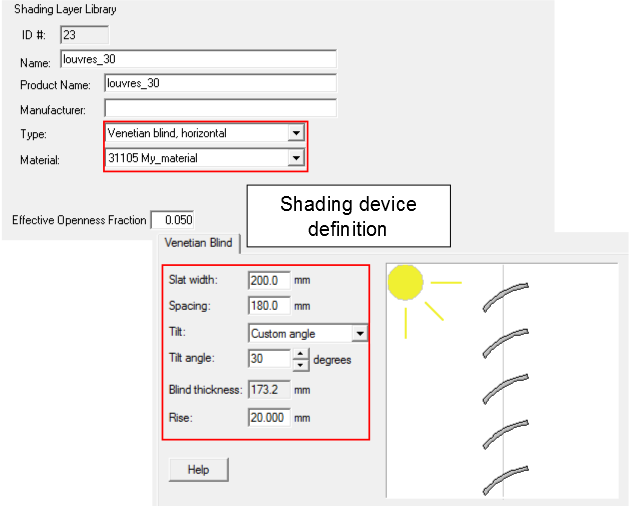
\includegraphics[width=0.6\textwidth]{shadinglibrary}
\caption{\label{img2:shading} Shading Layer Library }
\end{figure}

Once defined the fenestration system, it is required to set the optical calculation options in the software preferences (Figure \ref{img2:opticalcalc}). Checking the relative boxes, WINDOW gives in output the BSDF matrices of the complete fenestration system in a "xml" extension. In particular, it is possible also to have in output the BSDF data for both solar and visible band, remembering that for the daylighting simulations only the visible one is needed.

\begin{figure}[h]
\centering
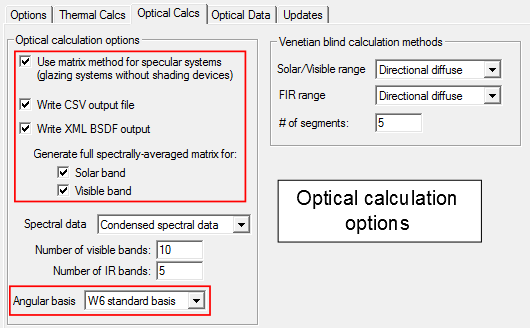
\includegraphics[width=0.6\textwidth]{opticalcalc}
\caption{\label{img2:opticalcalc} Optical preference setting - WINDOW 7.3}
\end{figure}

Particular attention should be paid to the angular basis option; this option defines the sky division in order to have a BSDF matrix 145x145 size, and to avoid error in the simulation. It is necessary to set the "W6 standard basis" (Figure \ref{img2:opticalcalc}) that correspond to the Klems division.
The BSDF file has to be saved with a name defined by an integer number which corresponds to a specific shading state in the TypeDLT simulation (e.g. 1.xml). Once created the BSDF file it is essential to locate it in a specific folder, where the TypeDLT can find it.
If the user will simulate a dynamic venetian system then will exist several BSDF files, one for each state of the blind.\\
\paragraph{Importing new window system in TRNSYS}
When a new window technology is created became necessary adding this new system to the Type56 window database. In TRNSYS will be add only the glazing part of the whole system, the shading will be considered apart from the glazing system using a shading factor (Fc) that represent the percentage of shaded area of the glazing surface. The tutorial \url{http://sel.me.wisc.edu/trnsys/downloads/tutorials_and_examples/window5/windowtutorial.pdf} will explain you how to add a new window in TRNSYS. 


\subsection{Google SketchUp}
It has been chosen to use different geometries for the simulations, that are a model for the thermal simulation and another for the daylighting simulation; this choice is due to the large simplification of the thermal model. In fact, the latter model is defined as plan surfaces that represent walls, instead, the daylighting model needs a volumetric geometry in order to consider the presence of shading objects, such as the walls thickness, pillars, but also furniture. This strategy is also useful if a building with a large number of thermal zone is simulated, in this case is not necessary redraw all the zones, but only the zone that we want to analyse with the daylighting simulation. This is possible because the simulations (thermal and daylighting) work on different geometries.  
Geometry can be drawn with Google SketchUp. The SketchUp's plug-in su2rad allows to export the SketchUp geometry (*.skp) in to Radiance geometry (*.rad) with a useful file structure. The possible ways to export in Radiance geometry are:

\begin{itemize}
\renewcommand{\labelitemi}{\tiny$\blacksquare$}
\item by group, for complex geometry;
\item by material, small number of files;
\item by layer, the more useful for geometry not so complex.
\end{itemize}

In order to simplify the procedure to define the reflection factor of the surfaces, two ways are suggested:
\begin{enumerate}
\item adding the material to the su2rad library, this procedure allows to set the the reflection coefficient within SketchUp
\item creating an alternative materials.rad file to be substitute to the one exported by su2rad.
\end{enumerate}

It is a good practice using standard material identifier that remember the name of the structural component (e.g. Internal\_walls). The exportation mode "by layer" is very useful if  at each layer a material/color is associated. In this way the user can control the coefficient of reflection of the surfaces without difficulties acting directly on all the surfaces contained in the layer especially working with the Radiance materials out of Skectch-up. With the "by group" mode is crucial to set well the materials before the export process. Otherwise, finding possible mistakes in the *.rad file becomes a hard task.\\
The name of the scene has to be defined considering the ID of the zone, that will be also the name of the folder containing the Radiance files (e.g. Zone1). As shown in Figure \ref{img2:rad}, su2rad generates a series of files. The folder "objects" contains all the elements that define the scene, each file takes the name of the layer (if the "by layer" mode is selected) and contains all the elements associate with that layer. Name the layer with the structural component (Figure \ref{img2:rad}) that compose the scene helps in maintain the order with the files and in the material/color association. Several folders contain file not used by the TypeDLT and in the next steps will be deleted.

\begin{figure}[h]
\centering
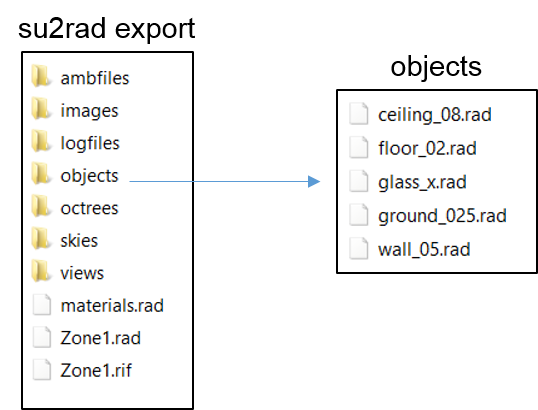
\includegraphics[width=0.6\textwidth]{rad}
\caption{\label{img2:rad} File rad exported by su2rad}
\end{figure}

The Zone1.rad and materials.rad files are the files managed by the user in order to set the inputs for the TypeDLT. The Zone1.rad file collects all the objects of the scene (Figure \ref{img2:zone1rad}) and the materials file in order to have few files during the creation of the octree file in Radiance. The materials.rad file contains the materials definition from SketchUp, in this file it is very easy to change the materials reflectance of the surfaces operating on the RGB channels in the last line of each material definition.

\begin{figure}[h]
\centering
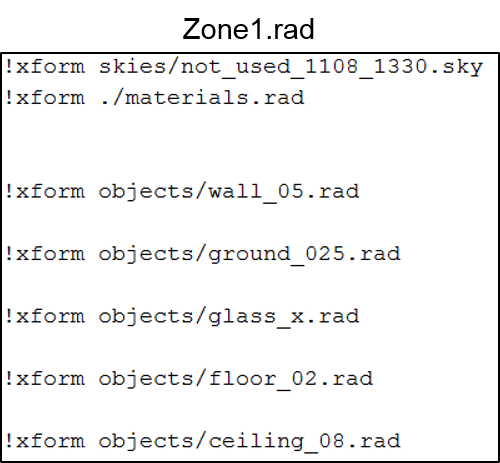
\includegraphics[width=0.4\textwidth]{zone1rad}
\caption{\label{img2:zone1rad} Content of the Zone1.rad file}
\end{figure}

\paragraph{Window and group of windows} 
An important annotation have to be done about the windows grouping. Windows that have the same orientation and that receive the incident daylight without discrepancies due to external obstruction can be grouped in the same layer. In this way, the windows grouped in the same layer will have the same shading control and will not be possible to control them separately.  \\
If you need more information on the windows grouping please consult the Appendix - Additional Consideration of the Three-Phase Method tutorial \cite{3ph_tut}.


\subsection{Manual tweaks}
First is required to bring the folder create by the su2rad in the project folder of the TRNSYS simulation, and name the folder Zone{\color{red} N} where {\color{red} N} is a positive integer number that define the zone analysed.\\
In figure \ref{img4:zone1} is shown an example of how locate the folder in the right place. The integer number that identifies the zone is the same number that has to be defined in Type's control panel under the input \textit{Zone ID} and the name of the Radiance scene, Zone1 in this case.
\begin{figure}[h]
\centering
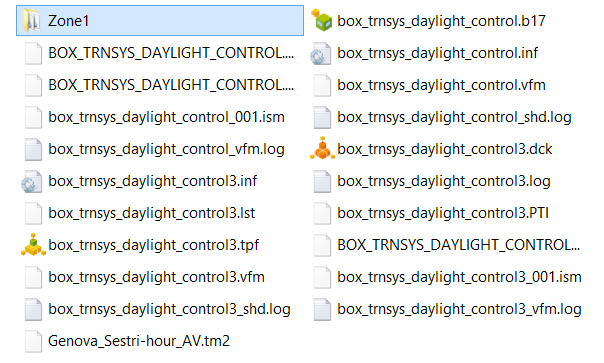
\includegraphics[width=0.7\textwidth]{zone1}
\caption{\label{img4:zone1} Positioning of the Radiance simulation folder in the TRNSYS project folder}
\end{figure}

Within the folder Zone1 is then necessary creating some folders: 
\begin{itemize}
\renewcommand{\labelitemi}{\tiny$\blacksquare$}
\item {\color{blue} data}, it will contain the matrices for the calculation, the file with the sensors grid and another subfolder:
\subitem{\tiny$\blacksquare$} {\color{blue} bsdf}, it will contain the bsdf data listed with integer numbers
\item {\color{blue} temp}, it will contain temporary files create during the matrices generation
\item {\color{blue} window}, it will contain the windows in the scene and a new file called win.vd
\end{itemize}

And deleting some other unused folder:
\begin{itemize}
\renewcommand{\labelitemi}{\tiny$\blacksquare$}
\item ambfiles
\item images
\item logfiles
\item octrees
\item skies
\end{itemize}

\begin{figure}[h] 
  \subfigure[]{% 
    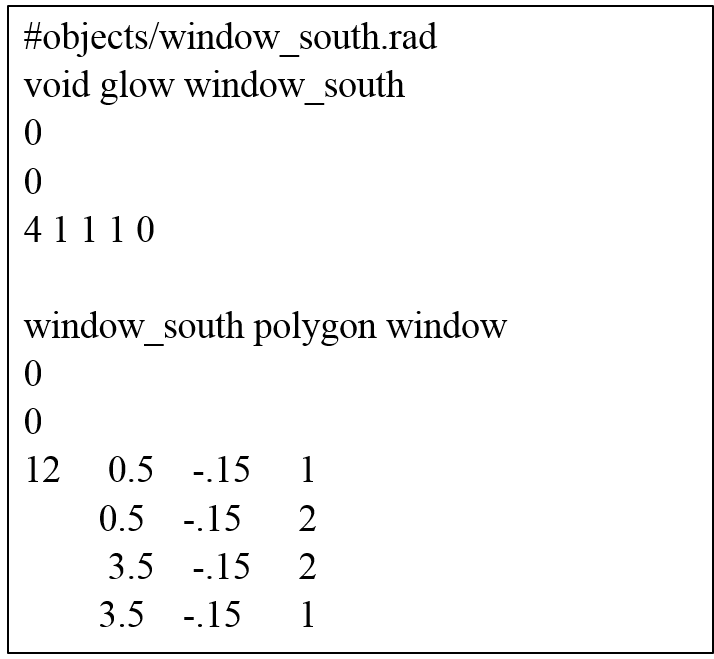
\includegraphics[width=.45\textwidth]{win} \label{img4:win} 
  }
  \subfigure[]{% 
    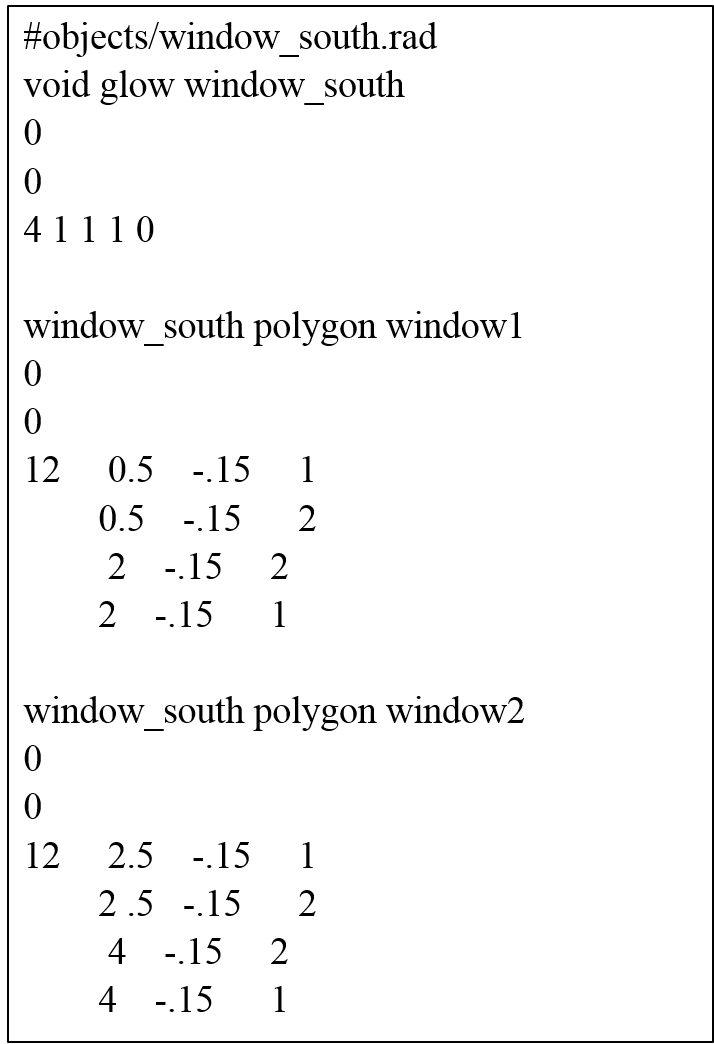
\includegraphics[width=.45\textwidth]{wingroup} \label{img4:wingroup} 
  } 
  \caption{\label{img4:winglow} Window file modified with the glow material for one window \ref{img4:win} and a group of two windows \ref{img4:wingroup}}
\end{figure}

In order to make available the input data for TypeDLT it is necessary to modify some files generated with SketchUp and to create a new one, which will collect all the windows in the scene. For this part, it is recommended to use a simple text editor. 3PM requires that the windows in the scene are a secondary light source, so that the user has to change the windows material in glow material, see Three-Phase Method tutorial for in-depth considerations \cite{3ph_tut}. To do this the user has to open the rad file containing the window/windows geometries and add in the heading of this file the glow definition as shown in figure \ref{img4:winglow}. Then, move the window.rad file from the "objects" folders to the "window" folder.

A new file called {\color{blue} win.vd} has to be created within the "window" folder. In this new file insert the number of windows/group of windows and the list of this windows/group of windows following a specific format: window modifier, view direction (vd) and view up (vp). The view direction is the window normal vector facing toward the outside of the room, the view up is the window up vector, vd and vu are always orthogonal.

Figure \ref{img4:windoworient} shows how to choose vd and vu from a sample geometry in which there is a window facing south. It is also shown how to report these information in the win.vd file for a window with modifier window\_south. 

Delete some rows from the rad file that contains all the objects into the scene, tutorial.rad in this case (figure \ref{img4:tutorial2}). In particular, the row that calls the sky definition and the window objects. In fact, TypeDLT creates at each time step a new sky file with the information contained in the weather file. And, the window/group of windows are used only for the matrices definition, in the calculation are then used the BSDFs data.

\begin{figure}[h]
\centering
\begin{minipage}[c]{0.6\linewidth}
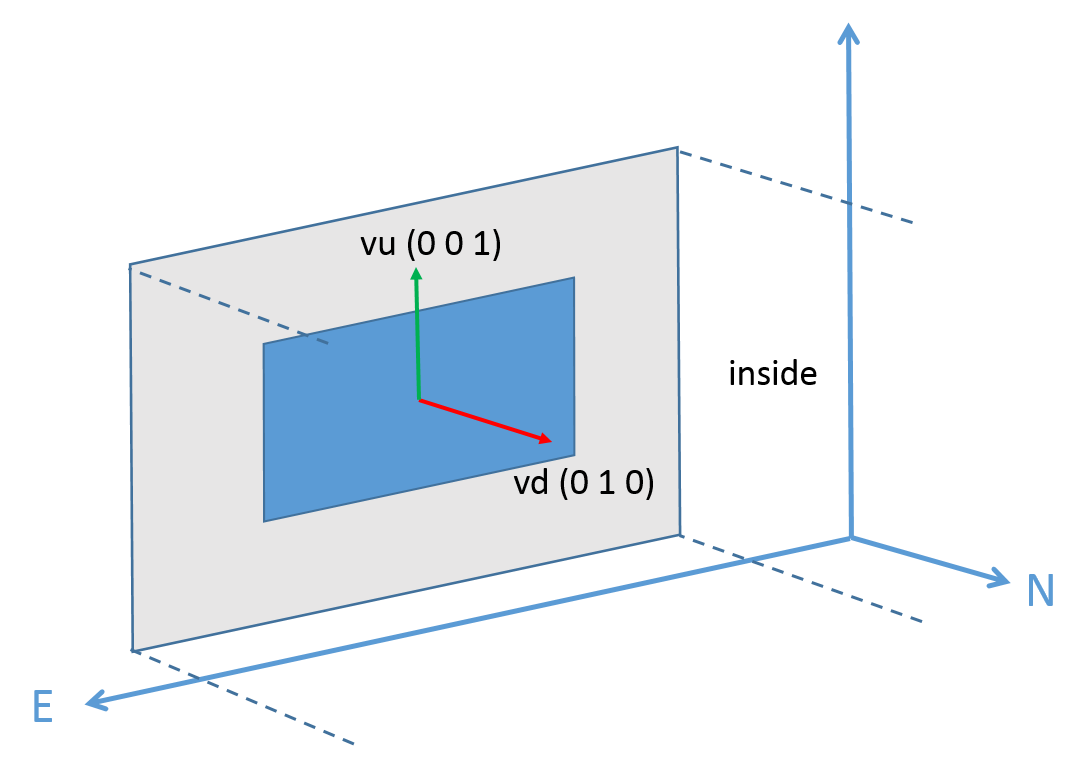
\includegraphics[width=1\textwidth]{windraw}
\end{minipage}
\quad
\begin{minipage}[c]{0.3\linewidth}
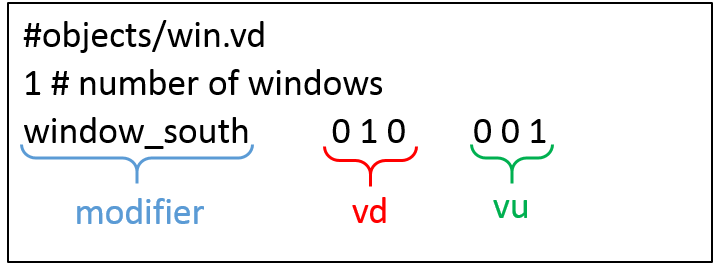
\includegraphics[width=1\textwidth]{winvd}
\end{minipage}
\caption{\label{img4:windoworient} New file with the list of windows in the scene and orientation of the vu and vd vectors}
\end{figure}


\begin{figure}[h]
\centering
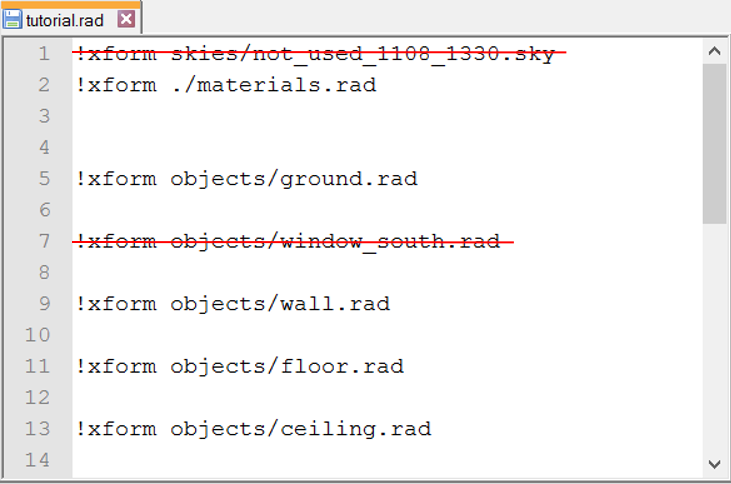
\includegraphics[width=0.5\textwidth]{tutorial2}
\caption{\label{img4:tutorial2} Contents of the tutorial.rad file}
\end{figure}

Add the file containing the sensors to be used in the simulations within the "data" folder with the name {\color{blue}grid.pts}. The format to follow is: x, y, z, dx, dy, dz where x, y and z are the three dimensional coordinates of the point and dx,dy and dz are the coordinates of the vector that define view direction of the sensor.
The example file (figure \ref{img4:grid}) is composed by row grid with 9 sensors located in the middle of the scene 1 meter from the window with a step of 0.5 m.

\begin{figure}[H]
\centering
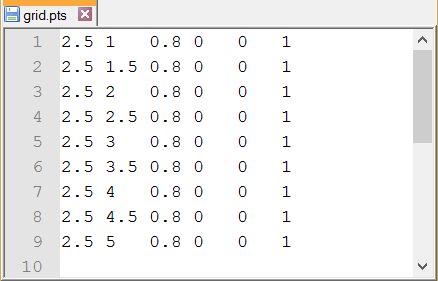
\includegraphics[width=0.5\textwidth]{grid}
\caption{\label{img4:grid} Format of the file containing the sensors grid}
\end{figure}


TypeDLT will create three files in the Zone folder: dmx.bat, vmx.bat and 3pm.bat. Those three batch files run the Radiance functions that generate respectively the daylighting matrix and the view matrix, which will be generate in the "data" folder (figure \ref{img4:zone1data}). With the latter batch file the sky is created and the daylighting simulation performed. Figure \ref{img4:zone1data} shows how the contents of the Zone folder look after the manual tweaks and a simulation in TRNSYS.


\begin{figure}[h]
\centering
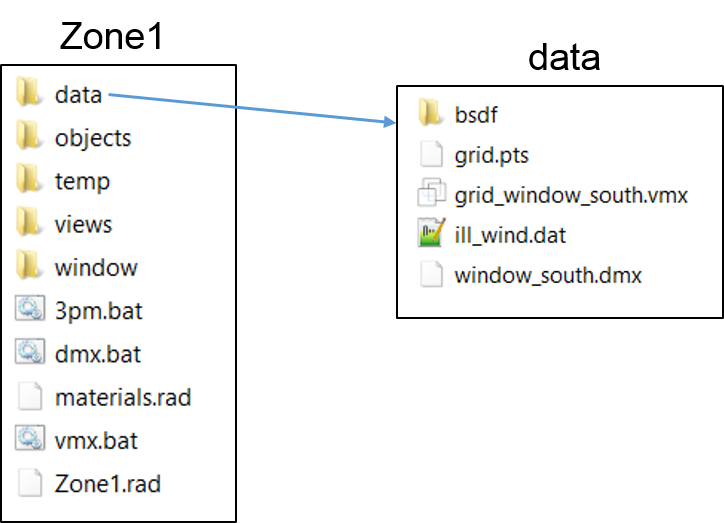
\includegraphics[width=0.5\textwidth]{zone1data}
\caption{\label{img4:zone1data} Contents of the Zone1 folder}
\end{figure}



\section{TRNSYS}
The creation of the thermal model can be done following the tutorial of TRNSYS3D plug-in for SketchUp in the TRNSYS documentation folder:
\begin{center}
....\textbackslash Trnsys17\textbackslash Documentation\textbackslash A4\_3DBuildingTutorial.pdf
\end{center} 

Locate the TypeDLT onto the TRNSYS deck. First, connect the following variable from the \textit{Weather data} Type: 
\begin{itemize}
\renewcommand{\labelitemi}{\tiny$\blacksquare$}
\item Latitude and Longitude 
\item Direct normal and diffuse horizontal illuminance
\item Month, day of the month and hour of the day
\end{itemize} 

\begin{figure}[h]
\centering
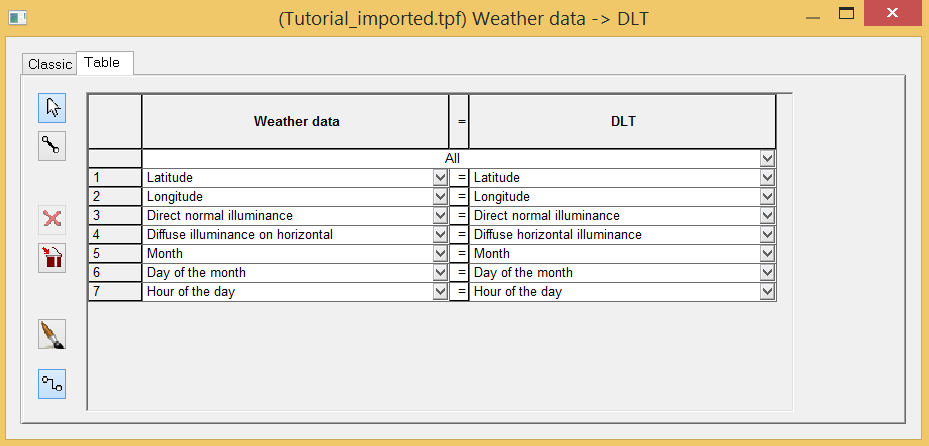
\includegraphics[width=0.7\textwidth]{DLTint}
\caption{\label{img5:DLTint} Connections between Weather data and TypeDLT}
\end{figure}


Double click on the TypeDLT icon, set the Zone ID that correspond to the integer number that you have assigned to the folder which contain the Radiance files on the input window. The default value in TRNSYS is 1 (Figure \ref{img5:DLTinput}).

\begin{figure}[h]
\centering
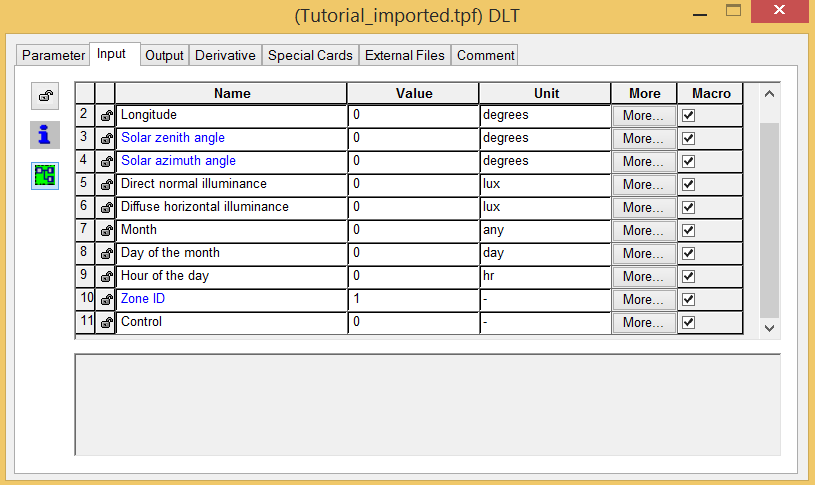
\includegraphics[width=0.7\textwidth]{DLTinput}
\caption{\label{img5:DLTinput} Input window TypeDLT }
\end{figure}


At this point, the TypeDLT is ready to simulate and the user can connect the Type's outputs and inputs following its needs.\\
\begin{figure}[h]
\centering
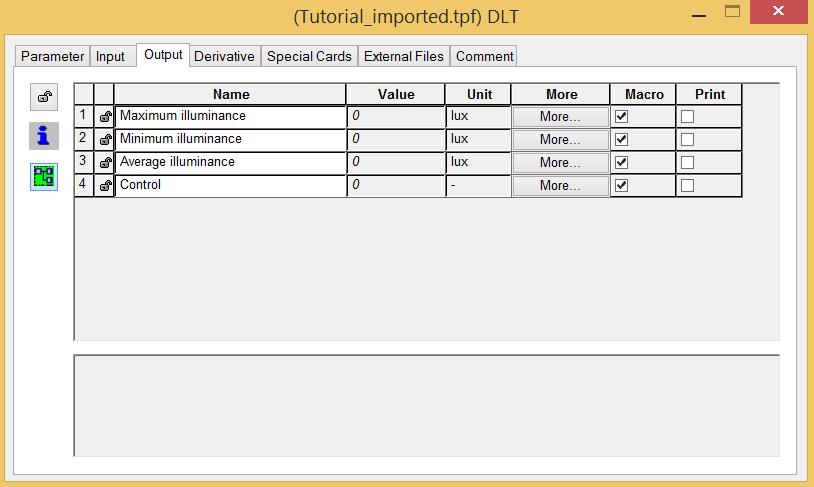
\includegraphics[width=0.7\textwidth]{DLToutput}
\caption{\label{img5:DLToutput} Output window TypeDLT }
\end{figure}
Once the TRNSYS deck is ready and the first simulation is run the view and daylighting matrices (see section \ref{sec:3ph} for theory) are generated and two terminal windows will be opened, Figure \ref{img5:matrices}.

\begin{figure}[h] 
\centering
  \subfigure[View matrix generation]{% 
    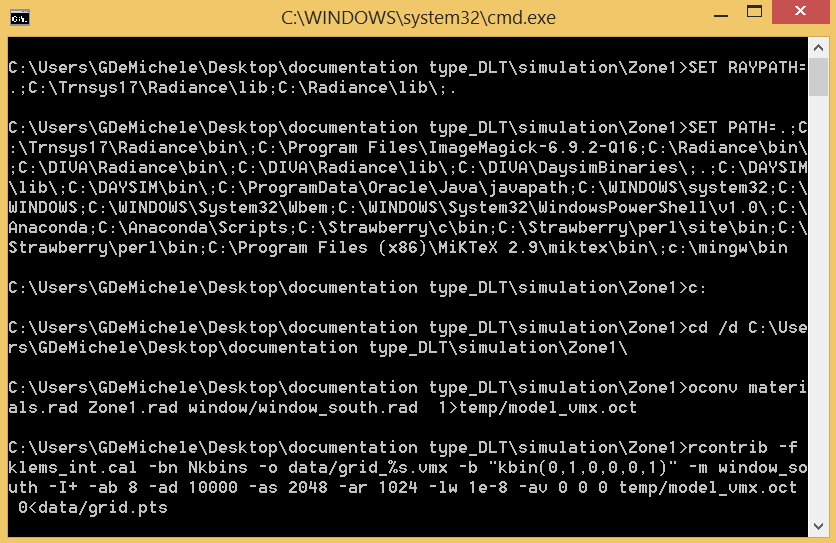
\includegraphics[width=.45\textwidth]{vmx} \label{img5:vmx} 
  } 
  \subfigure[Daylighting matrix generation]{% 
    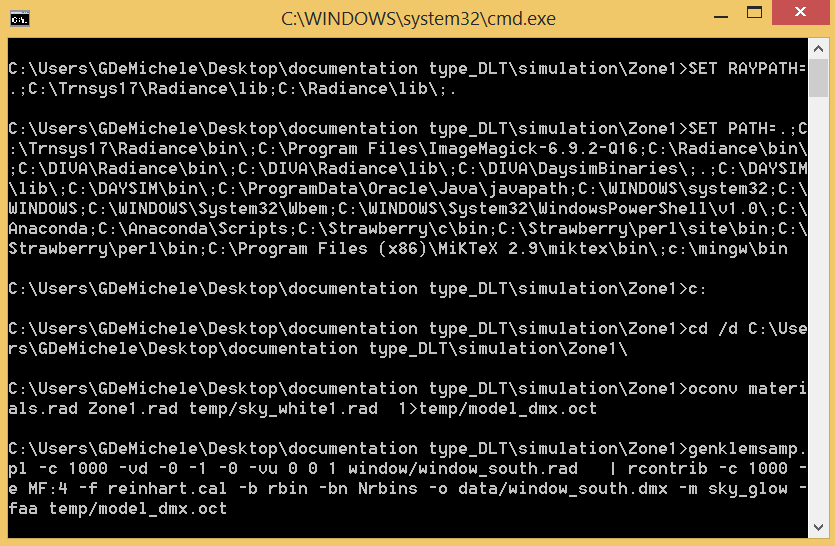
\includegraphics[width=.45\textwidth]{dmx} \label{img5:dmx} 
  }
  \caption{\label{img5:matrices} Terminal windows opened for the view and daylighting matrix generation}
\end{figure}

\begin{figure}[H]
\centering
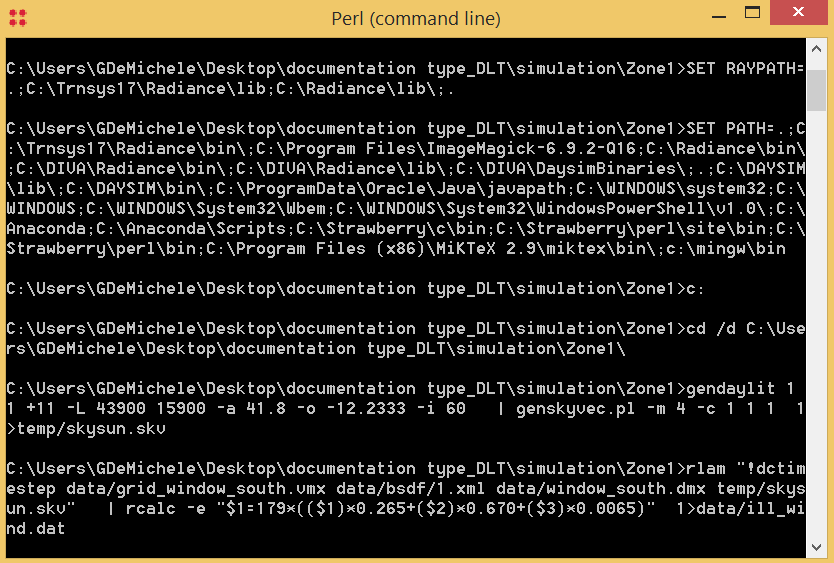
\includegraphics[width=0.5\textwidth]{3pm_t}
\caption{\label{img5:3pm} Terminal window - Sky vector generation and matrix multiplication }
\end{figure}

The vmx and dmx matrices generation requires several minutes depending also by the complexity of the geometry and the number of windows in the scene. Once the matrices are crated it is not necessary to regenerate them at each time-step and for the next simulations of the same Radiance scene. At each time-step will be created the sky vector and performed the matrices multiplication (Figure \ref{img5:3pm}) that require few seconds.
It is very important to know that the *.vmx and *.dmx files generated are not overwrite in any case, therefore if you need to regenerate these files delete them manually in the folder "data".\\

\subsection{Radiance parameters}
The Radiance parameters that define the quality of the simulation and the results accuracy can not be modified yet. At the state of art the simulation is performed with fixed parameters, that has been chosen according to the Three-Phase Method tutorial. The default values for the view matrix calculation are:

\begin{center}
-I+ -ab 12 -ad 50000 -lw 2e-5
\end{center}

where \cite{rad_tut}:
\begin{itemize}
\renewcommand{\labelitemi}{\tiny$\blacksquare$}
\item I, boolean switch to compute irradiance rather than radiance
\item ab, ambient bounce, is the maximum number of diffuse bounces computed by the indirect calculation
\item ad, ambient division, the error in the Monte Carlo calculation of indirect illuminance will be inversely proportional to the square root of this number
\item lw, limit the weight of each ray to a minimum
\end{itemize}

The default values for the daylighting matrix calculation are: 
\begin{center}
-c 1000 -e MF:4
\end{center}
where \cite{3ph_tut}: 
\begin{itemize}
\renewcommand{\labelitemi}{\tiny$\blacksquare$}
\item c is the number of sample rays produced per Klems division
\item -e allows to change the sky division. In this case MF:4 - 2305 divisions
\end{itemize}

In order to change these values the user has to modify them in the C\texttt{++} code and repeat the dll compilation procedure.
\begin{thebibliography}{1}

\bibitem{trnsys} TRNSYS, {\em URL:\url{http://www.trnsys.com/}}.

\bibitem{radiance} G. Ward, J, {\em The RADIANCE Lighting Simulation and Rendering System}, 21st Annu. Conf. Comput. Graph. Interact. Tech., pp. 459-472, 1989.
  
\bibitem{3ph1}  M. Saxena, G. Ward, T. Perry, L. Heschong, and R. Higa, {\em DYNAMIC RADIANCE - PREDICTING ANNUAL DAYLIGHTING WITH VARIABLE FENESTRATION OPTICS USING BSDF}, Fourth National Conference of IBPSA-USA, pp. 402-409, 2010. 

\bibitem{3ph2}G. Ward, R. Mistrick, E. S. Lee, A. McNeil, and J. C. Jonsson, {\em Simulating the Daylight Performance of Complex Fenestration Systems Using Bidirectional Scattering Distribution Functions within Radiance}, Leukos, vol. 7, pp. 241-261, 2011.

\bibitem{3ph_tut}A. McNeil, {\em The Three-Phase Method for Simulating Complex Fenestration with Radiance}, LBNL, 2014.

\bibitem{bsa}G. De Michele, U. Filippi Oberegger, L. Baglivo, {\em Coupling dynamic energy and daylighting simulations for complex fenestration systems}, BSA 2015 2nd IBPSA-Italy Conference, Bolzano-Bozen, pp. 289-296, 2015.

 
\bibitem{rad_tut} A. McNeil,  G. Antonutto, {\em  Radiance premier }, URL: \url{http://www.radiance-online.org/learning/tutorials/radiance-primer.pdf}.
 

\end{thebibliography}

\end{document}